\documentclass[12pt]{article}
\usepackage{amsmath}
\usepackage{refstyle}
\usepackage{caption}
\usepackage{graphicx}
\usepackage{multirow}
\usepackage{csvsimple}
\usepackage{pgfplotstable}
\pgfplotsset{compat=1.17}
\usepackage{booktabs}
\usepackage{geometry}
\geometry{ a4paper, total= {170mm, 257mm}, left=20mm, top=20mm,}
\usepackage{cite}
\usepackage{amssymb,amsfonts}
\usepackage{algorithmic}
\usepackage{textcomp}
\usepackage{xcolor}
\usepackage{cuted}
\usepackage{capt-of}
\usepackage{multicol}
\setlength{\columnsep}{0.60cm}
\title{\textbf{Assignment 1}}
\author{Bhushan Shah \\ MIS : 112103129}
\date{8th November 2022}
\pagenumbering{roman}
\begin{document}
\maketitle
\newpage
\tableofcontents
\clearpage
\section{Introduction}
\emph{Hello, This is my first document.}
\subsection{Quadration Equation}
Question : Solve the following quadratic equation :- 
$x ^ 2 + 5x + 6 = 0$
\\
\\
$x ^ 2 + 5x + 6 = 0$
$\\ x ^ 2 + 3x + 2x + 6 = 0$
$\\ x(x + 3) + 2(x + 3) = 0$
$\\ (x + 3) * (x + 2) = 0$
$\\ x + 3 = 0$ or $x + 2 = 0$
$\\ x = -3$ or $x = -2$
\clearpage
\begin{large}
\section{Maths question paper}
\begin{center}
\textbf{College of Engineering, Pune Technological University}
\end{center}
Subject - Maths\hspace{5cm} Duration - 1 hr 30 min\\
Date - 15/11/22\hspace{5cm} Max marks - 40
\subsection*{Section A}
\noindent Q1) Show that the following limits exist and find them:
\begin{equation*}
(a)\lim_{n\to\infty} \frac{n!}{n^n}\hspace{2cm}
(b) \lim_{n\to\infty} (\frac{n}{n^2 + 1} + \frac{n}{n^2 + 2} + ... + \frac{n}{n^2 + n})
\end{equation*}
\begin{equation*}
(c) \lim_{n\to\infty} \frac{sin(n)}{n^2}\hspace{1cm}
(d) \lim_{n\to\infty} sin(\frac{1 + 2 + ... + n}{n^2})
\end{equation*}
\\\\
\noindent Q2) Prove that the following sequences are convergent by showing that they are mono-
tone and bounded. Also find their limits\\
\begin{align*}
&(a)a_1 = 2,a_{n+1} = \frac{1}{2}(a_n + \frac{2}{a_n}), \forall n \ge 1\\
\vspace{1mm}
&(b)a_1 = \sqrt{2},a_{n+1} = \sqrt{a_n + 1}), \forall\ge 1\\
\vspace{1mm}
&(c)a_1 = 2,a_{n+1} = a_n + \frac{1}{2^n}), \forall n \ge 1\\
\end{align*}
Q3) Find the radius and the interval of convergence of the following power series.

\begin{equation*}
(a) \sum_{n = 1}^{+\infty} (-1)^{n + 1} \frac{n^2}{n^4 + 1} \hspace{2cm} (b) \sum_{n = 1}^{+\infty} \frac{(-1)^n}{1 + \sqrt{n}}
\end{equation*}
\\\\
\noindent Q4) Find the volumes of the solids generated by revolving the regions bounded by the
lines and curves about the y- axis.\\
The region is enclosed by :-
\begin{equation*}
 x = 2sin(2y), 0 \geq y \geq \pi /2, x = 0. \hspace{1cm}and \hspace{1cm} x = \sqrt{cos(\frac{\pi x}{4})}
\end{equation*}
\subsection*{Section B}
Q1) Evaluate the following improper integrals :-
\begin{equation*}
(a) \int_{-1}^{\infty} \frac{\,dx}{\sqrt{x^2 +5x + 6}} 
\end{equation*}
\begin{equation*}
(b) \int_{0}^{\infty} \frac{(xsin(x) + x^3)^{2}}{\sqrt{x}}
\end{equation*}
Q2) Prove the following reduction formulae and state the values of n for which they are valid. Note that m,n are nonnegative integers.\\
$(a) If U_{n} = \int_{0}^{\pi} \theta cos(\theta)^n$ then prove that $U_{n} = \frac{-1}{n^2} + \frac{n}{n - 1}U_{n - 2}$\\\\
(b)$If I_{n} = \int_{\frac{\pi}{4}}^{\pi} cot(x)^n \,dx$ then prove that $I_{n} = \frac{1}{n - 1} - I_{n - 2}$ Hence evaluate $I_{6}$\\\\
Q3)If A = 
$
\begin{bmatrix}
1 & 2 & 3\\
3 & 4 & 0\\
12 & -1 & 0
\end{bmatrix}
$
and $A^{-1} = \frac{A^2 + cA + d}{6}$ then the values of c and d are respectively is -\\ 
(A) -6, -11 \hspace{5cm} (B) 6,11\\
(C) -11, 11 \hspace{5cm} (D) None\\
Q4)Given
$
3
\begin{bmatrix}
x & y\\
z & w
\end{bmatrix}
$
=
$  
\begin{bmatrix}
x & 6\\
-1 & 2w
\end{bmatrix}
$
+ 
$
\begin{bmatrix}
4 & x + y\\
z + w & 3
\end{bmatrix}
$
, determine the values of x, y, z, w.(Hint: Use Comparison method)\\\\
Q5) If A = 
$
\begin{bmatrix}
3 & -2\\
4 & -2
\end{bmatrix}
$
and I = 
$
\begin{bmatrix}
1 & 0\\
0 & 1
\end{bmatrix}
$
, find k so that $A^2  = kA - 2I.$
\clearpage
\section{Introducing images in Latex}
\subsection{Aston Martin}
Aston Martin is a modern, exclusive sports car brand with a unique heritage instantly recognised around the world. Founded in 1913 by Lionel Martin and Robert Bamford, Aston Martin is acknowledged as an iconic global brand synonymous with style, luxury, performance and exclusivity. The British marque fuses the latest technology, time honoured craftsmanship and graceful styling to produce a range of critically acclaimed sports cars. After celebrating its 100th birthday in 2013, Aston Martin is looking firmly forward to its next century of “Power, Beauty and Soul”.The first Aston Martins were created with a distinctive and individual character, handcrafted to the highest of standards, and capable of exceeding all performance expectations. Over the past century, the marque has stayed true to the original values of Lionel Martin.

\begin{figure}[h]
\centering
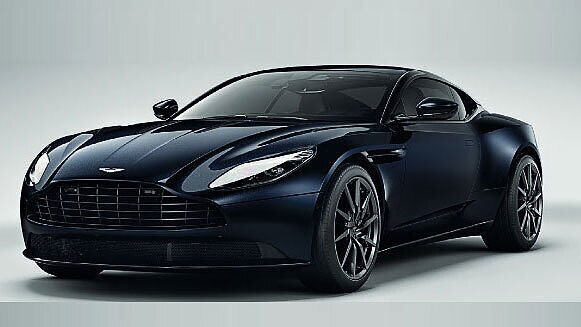
\includegraphics[scale=0.5]{AstonMartin.jpg}
\caption{Aston Martin}
\label{fig : Aston Martin}
[\ref{fig : Aston Martin}] shows classic Aston Martin car. It was launched in 2018 and has been loved by the customers even since.\\
\end{figure}
\clearpage
\subsection{Eiffel Tower}

Image result for what is eiffel tower
The Eiffel Tower—or as the French call it, La Tour Eiffel—is one of the world's most recognizable landmarks. The tower was designed as the centerpiece of the 1889 World's Fair in Paris and was meant to commemorate the centennial of the French Revolution and show off France's modern mechanical prowess on a world stage.\\
\begin{figure}[h]
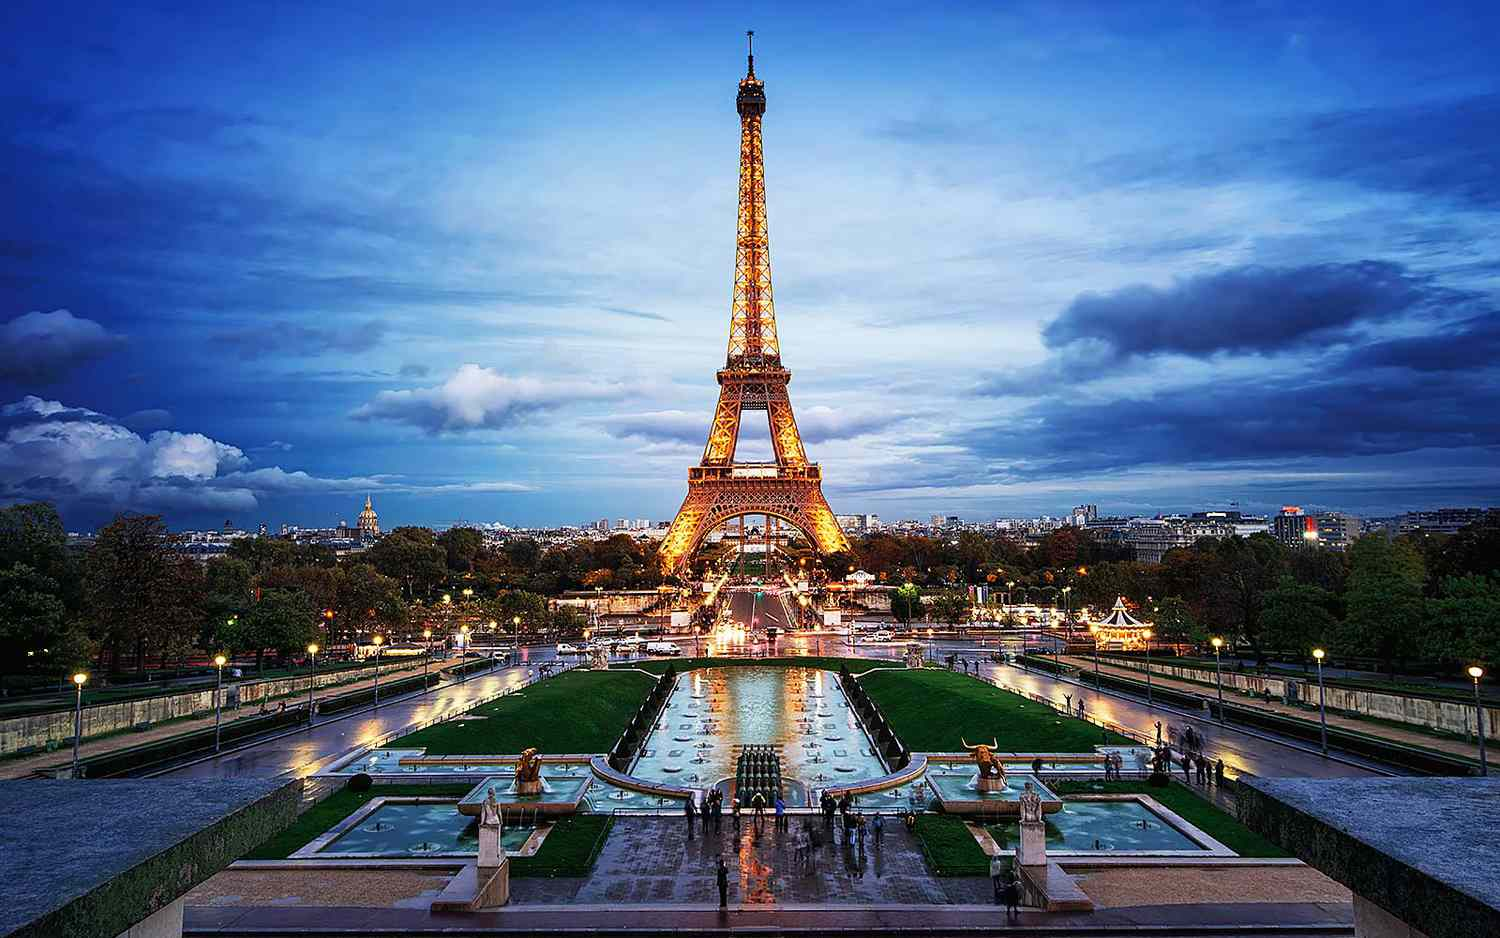
\includegraphics[scale=0.23]{EiffelTower.jpg}
\caption{Eiffel Tower}
\label{fig : Tower}
[\ref{fig : Tower}] above shows the image of one of seven wonders of the world Eiffel Tower. It attracts many tourist and is the major source of income for most of the people living in that area.
\end{figure}

\section{Introducing tables in Latex}
\subsection{Table1}
\begin{tabular}{|c|c|c|c|c|c|c|c|c|c|}
\hline \hline
Audio & Audibility & Decision  & \multicolumn{7}{|c|}{Sum of Extracted Bits}\\
\hline
\multirow{2}{*}{Police} & \multirow{2}{*}{5} & soft & 1 & -1 & 1 & 1 & -1 & -1 & 1\\ 
&  & hard & 2 & -4 & 4 & 4 & -2 & -4 & 4\\ \hline
\multirow{2}{*}{Beethoven} & \multirow{2}{*}{5} & soft & 1 & -2 & 1 & -1 & -3 & 2 & 5\\
 &  & hard & 2 & 4 & 4 & 5 & 1 & -4 & -5\\ \hline
\multirow{2}{*}{Police} & \multirow{2}{*}{5} & soft & 1 & 1 & 2 & -1 & 1 & 2 & 1\\
 &  & hard & 2 & 3 & 5 & -3 & -2 & 2 & 6\\
\hline \hline
\end{tabular}
\vspace{1cm}
\\
Noise pollution has been recognized as one of the major hazard that impacts the quality of life.Noise pollution has been recognized as one of the major hazard that impacts the quality of life all around the world. Because of the rapid increase in technology, noise pollution has reached to a disturbing level over the years which needs to be studied and controlled to avoid different health effects.\\\\
\subsection{Table using csv file}
\begin{table}[h!]
\caption{Table imported through pgfplotstable}
\label{csvTable}
\begin{center}
\pgfplotstabletypeset[
	col sep=comma,
	columns/Month/.style = {string type},
	every head row/.style = {
		before row=\hline
		after row=\hline
	},
	every last row/.style={after row=\bottomrule},
]{sheet.csv}
\end{center}
\end{table}
\vspace{0.7cm}
Above table shows the monthly expense and profit of a local store. Keeping track of the expense and profit makes them aware of how the bussiness is doing and how to solve any issues if any.
\section{Bibliography}
\subsection{Black Holes}
A black hole is a region of spacetime where gravity is so strong that nothing, including light or other electromagnetic waves, has enough energy to escape it ~\cite{1}.The theory of general relativity predicts that a sufficiently compact mass can deform spacetime to form a black hole.~\cite{2, 3} The boundary of no escape is called the event horizon. Although it has a great effect on the fate and circumstances of an object crossing it, it has no locally detectable features according to general relativity.~\cite{4} In many ways, a black hole acts like an ideal black body, as it reflects no light.~\cite{5, 6} Moreover, quantum field theory in curved spacetime predicts that event horizons emit Hawking radiation.
\subsection{Reference}
\begin{thebibliography} {}
\bibitem {1} Wald 1984, pp. 299–300
\bibitem {2} Wald, R. M. (1997). "Gravitational Collapse and Cosmic Censorship". In Iyer, B. R.; Bhawal, B. (eds.). Black Holes, Gravitational Radiation and the Universe. Dordrecht: Springer. pp. 69–86. arXiv:gr-qc/9710068. doi:10.1007/978-94-017-0934-7. ISBN 978-9401709347.
\bibitem {3} Overbye, Dennis (8 June 2015). "Black Hole Hunters". NASA. Archived from the original on 9 June 2015. Retrieved 8 June 2015.
\bibitem {4} Hamilton, A. "Journey into a Schwarzschild black hole". jila.colorado.edu. Archived from the original on 3 September 2019. Retrieved 28 June 2020.
\bibitem {5} Schutz, Bernard F. (2003). Gravity from the ground up.
\bibitem {6} Davies, P. C. W. (1978). "Thermodynamics of Black Holes".
\end{thebibliography}
\end{large}
\pagebreak
\section{Research Paper}
\begin{huge}
\begin{center}
Application of Hierarchical Temporal Memory Theory for Document Categorization
\end{center}
\end{huge}
\vspace{0.2cm}
\begin{center}
\begin{Large}
Deven Shah \hspace{2cm} Pinak Ghate \hspace{2cm} Manali Paranjape\\
\end{Large}
deven.shah@gmail.com \hspace{0.5} pinakghate@gmail.com \hspace{0.5cm} paranjape.manali@gmail.com
\end{center}
\begin{multicols}{2}
\begin{abstract}
 The current work intends to study the performance
of the Hierarchical Temporal Memory(HTM) theory for auto-
mated classification of text as well as documents. HTM is a
biologically inspired theory based on the working principles of
the human neocortex. The current study intends to provide
an alternative framework for document categorization using
the Spatial Pooler learning algorithm in the HTM Theory. As
HTM accepts only a stream of binary data as input, Latent
Semantic Indexing(LSI) technique is used for extracting the
top features from the input and converting them into binary
format. The Spatial Pooler algorithm converts the binary input
into sparse patterns with similar input text having overlapping
spatial patterns making it easy for classifying the patterns into
categories. The results obtained prove that HTM theory, although
is in its nascent stages, performs at par with most of the popular
machine learning based classifiers.\\
Index Terms - Hierarchical Temporal Memory, Document Cat-
egorization, Machine Learning, Spatial Pooler, Latent Semantic
Indexing, NuPIC, Supervised Learning
\end{abstract}
\subsection{Introduction}
One of the elemental forms of document processing includes
classification. Since the last couple of years, it is in demand
because of the increasing availability of data in digital format
which has resulted into the requirement of systematization of
that data. Manual organization of huge data can be tedious
if strict time constraints are set, increasing the necessity of
automated document classification. The contexts of words in
the documents play a very important role in deciding the
category of the document. The human brain is very effective
in consideration of contexts in the incoming information for
taking the appropriate action.\\
The principles of HTM theory can be used to meet the
requirements of organizing of data. HTM takes inspiration
from the mammalian brain which has been evolving over
millions of years and is able to process data efficiently. As
HTM is biologically plausible, it is based on simple rules and
not complex mathematics. HTM theory is being developed by
a US based company called Numenta, Inc.
\subsection{Related Work}
Some of the conventional methods for text/document clas-
sification are mentioned below:
\subsubsection{Naive Bayes}
The Naive Bayes classifier is a probabilistic classifier and is
based on the Bayes theorem. It works well with small samples
of data. The posterior probability of a particular document
belonging to various classes is calculated. The document is
assigned to the class with the highest posterior probability. The
Naive Bayes classifier assumes strong independence between
the features. This is a major limitation of this classifier and
hence has low performance in cases where the features are
correlated.~\cite{1}
\subsubsection{Support Vector Machines}
Support Vector Machines (SVMs) are supervised machine
learning algorithms. In case of a multi class problem, first
the problem has to be decomposed into two separate class
problems as SVM can work only with binary classification
problem. They will probably give poor results when total
number of samples are very less than the total number of
features. In comparison with decision making classifier and
logistic regression, SVM takes more time for computation. ~\cite{1}
\subsubsection{K-Nearest Neighbour}
K-Nearest Neighbour (KNN) is used for classification of
objects by calculating the distance of training samples from
each object. KNN classification is a simple and widely used
approach for text classification. However, it is computationally
intensive and classification time is high ~\cite{1}. Also, it is difficult
to find the ideal value of k.~\cite{2}

\subsubsection{Convolutional Neural Network}
Convolutional Neural Network (CNN) works well with static text classifications. CNN is a type of feed forward neural network, comprising of neurons with trainable weights
and biases~\cite{3}.
\end{multicols}
\begin{figure}[h]
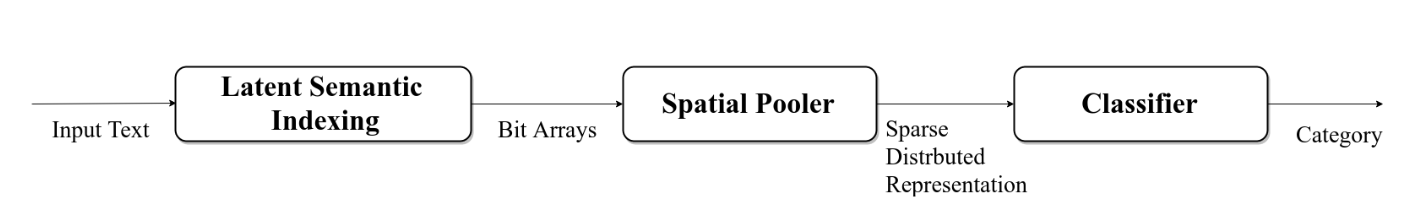
\includegraphics[scale=0.36]{image1.png}
\captionof{figure}{System Architechture Diagram}
\end{figure}
\begin{multicols}{2}
CNN comprises of a number of convolutional layers with nonlinear activation functions like ReLU or tanh applied to the results. CNN suffers from the limitations of the requirement of large data and big processing power to be able to predict accurately.\\HTM theory is primarily used for Classification, Prediction and Anomaly Detection purposes. One of its application for
Classification is mentioned above:
\subsubsection{Land - forms Classification}
As HTM based models have a common learning algorithm,
it can be used for classifying images. HTM theory has been
used for classifying different land-forms like trees, roads,
buildings and farms using the images obtained from satellites.
The framework used achieved an accuracy of 90.4\%, \cite{4} which
is at par with the conventional machine learning techniques for
image classification.\\
Since HTM theory can be used for image classification
purposes, it can hold a promise to classify text/documents.
\subsection{Overview of Herarchial Temporal Memory}
HTM is a theory which seeks to apply the structural as well
as algorithmic properties of the neocortex to machine learning
problems ~\cite{5}. The neocortex proves to be the center of intelli-
gence in the mammalian brain. It is responsible for processing
complex activities such as communication, planning and pre-
diction. Structurally, neocortex is a 2 mm thick tissue divided
into a number of different regions. A region is a network of
interconnected neurons ~\cite{5}. This attributes to the presence of
input connections from different sensory organs 
~\cite{6,7} like
eyes, ears etc. The term “Hierarchical” in the theory is owing
to the fact that, HTM network contains a hierarchy of levels
arranged in the pyramid-like structure. These levels are present
in the form of regions that are again composed of columns
which finally consist of neurons. These neurons need not be
physically arranged in a hierarchy, but are logically arranged in
the hierarchical format. The lower levels in hierarchy represent
data having lower abstraction/complexity. As we go higher
in the hierarchy, the data abstraction stored in the memory
increases. Time plays a crucial role in the way data is stored in
mammalian brain. “Temporal” implies that the HTM network
takes into consideration the sequence of the incoming data. A
continuous stream of input data is aptly learned as spatial and
temporal sequences.\\
A remarkable property of the neocortex is that the input
from all the sensory organs is processed in the same manner.
Hence, it has a common learning algorithm for inputs from
all types of sensory organs ~\cite{5}.

\subsubsection{Structure of a Neuron}\label{AA}
Inside the mammalian brain, neurons play a central role in
information handling. Some relevant parts of the neuron for
our study are mentioned below.\\
1) Proximal Dendrites: Proximal dendrites are in close
proximity to the cell body. The proximal dendrites are con-
nected directly to the inputs from the sensory organs.\\
2) Distal Dendrites: Distal dendrites are the ones that are
afar from the cell body. The distal dendrites have connections
with various other neurons in the neocortex. Majority of the
connections to the axon are from distal dendrites as compared
to the connections made by proximal dendrites ~\cite{8}.\\
3) Synapse: A synapse is a connection between an axon of
one neuron and dendrite of the other. The ongoing process of
breaking and reforming these synapses between cells results
in learning of new data and thus gradually forgetting the old
one.\\
There is a permanence value associated with every synapse
and a threshold linked with every neuron. Thus, for a neuron
to get activated, the total number of synapses with permanence
values higher than the threshold value must be more than the
stimulus threshold.
\subsubsection{Sparse Distributed Representation}
Though the neocortex contains billions of neurons in highly
interconnected manner, only a tiny fraction of them are active
for a particular input ~\cite{9}. Hence, only small percentage of
active neurons are responsible for representing the input in-
formation. This is called as Sparse Distributed Representation
(SDR). Even though single activated neuron has the potential
to convey some meaning, the full information can only be
conveyed when it is interpreted within the context of other
neurons. As the information is spread across a tiny percentage
of the active bits, SDRs are more noise tolerant than dense
representations, making them ideal for text processing.

\subsubsection{Spatial Pooler}
HTM includes two important parts - Spatial Pooler (SP) and Temporal Pooler (TP). Spatial Pooler, also known as Pattern Memory, has been emphasized in this study.\\
The neurons in the neocortex are arranged in columns, which represent features of the input. Every neuron in a particular column, which represent different context for an input, is connected to specified number of bits in the input bit array. The selection of bits t be connected to the neurons in a particular column is random. The bits which are connected
to a particular column are known as a potential pool of that particular column. Connections between input bit and the column neuron is called as a synapse. Every synapse has a
value associated with it known as permanence value similar to that of a mammalian brain. Permanence value is always in the range of 0 and 1. There is a threshold value associated
with synapse’s permanence.\\
If the permanence value of a synapse associated to an input bit is greater than the threshold, the activation of the column ofneurons is influenced by the input bit. The permanence value of a synapse is adjusted in the learning phase.\\
The main role of SP in HTM is finding spatial patterns in
the input data. It is decomposed into three stages:\\
1) Overlap: In this stage, overlap score of each column
is calculated. Overlap score is the count of active bits in the
potential pool of a particular column having permanence value
greater than the threshold.\\
2) Inhibition: The columns are sorted according
to their overlap scores from highest to lowest. A
particular fraction (in our study, 0.5\%, Table I,
N umActiveColumnsP erInhArea) of the top columns
is selected (also called as active columns or the winning
columns) for the learning phase. Rest other columns are
inhibited from learning.\\
3) Learning: During Learning, the permanence value of
the synapses in the potential pool of the winning columns is
incremented (by synPermActiveInc, Table I) or decremented
(by synPermInactiveDec, Table I). When the active column
is connected to an active bit then the permanence value of
the synapse corresponding to that active bit is incremented.
However, when the active column is connected to an inactive
bit then the permanence value of the synapse corresponding to
that inactive bit is decremented. This is the result of column
expecting that bit to be active. The synapse permanence is
decremented as a punishment.

\subsection{Implementation}
The flowchart in figure 1 is our high-level architecture
diagram for document categorization. As the mammalian brain
requires electrical signals for learning, the learning algorithm
i.e., Spatial Pooler also requires bit patterns for processing.
So, to convert text into bit arrays, Latent Semantic Indexing
(LSI) technique is used, which converts semantically similar
sentences into similar bit arrays. These bit arrays (which need
not be sparse) are fed to the Spatial Pooler where it simulates
the working of neurons in the brain and gives SDR as the
output. The active bits in the SDR represent the neurons which
get activated in the Spatial Pooler. Since semantically similar
text belong to the same category, it is easy to classify the text
into different categories.

\subsubsection{Latent Sematic Indexing}
As HTM theory is modelled after the mammalian brain,its input also should be in accordance with the input formatreceived by the brain. The brain receives input in the formof electrical signals which correspond to bit arrays. Latent
Semantic Indexing(LSI) helps in determining hidden featuresin documents ~\cite{10}. Thus the technique is used to extract thecontextual-usage meaning of words from the documents ~\cite{11}.
The LSI framework consists of 3 steps which are mentioned below.
\end{multicols}
\begin{figure}[h]
\begin{center}
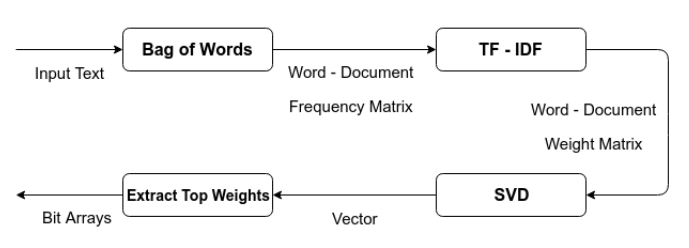
\includegraphics[scale=0.38]{image2.png}
\caption{Latent Semantic Indexing framework}
\end{center}
\end{figure}
\begin{multicols}{2}
1) Preprocessing of input data: In the initial step, the
input text is tokenized and stopwords are removed from
every document of the corpus1 . Each term in the text is then
represented as a tuple containing term-id and term frequency.
A matrix is created in which the rows denote the unique terms
and the columns denote the documents. Every cell denotes
the term count in the corresponding document. The matrix
of term-frequency counts obtained from the term document
matrix is then modified using the TF-IDF technique so as to
give more weight to rare terms compared to common terms
across documents and also to frequently occurring terms in a
particular document. The formula for weighing each term can
be represented as,\\
\begin{equation}
DocumentTermWeight = f_{t,d} \times ln(\frac{N}{n_{t}})
\end{equation}
where,\\
$f_{t,d}$ : count of term t in document d\\
N : the total count of documents\\
nt : the count of documents having term t\\
The term-document matrix gets modified to contain weights
of each term in a given document. The dimensionality reduc-
tion of this matrix is done using Singular Value Decomposition
(SVD).\\
2) Singular Value Decomposition: LSA uses SVD for generating the vectors of a particular text ~\cite{12}, ~\cite{13}. The matrix X(term-document) is used to calculate two matrices. These are,\\
\begin{equation}
Y = \mathbf{X}^T X
\end{equation}
\begin{equation}
Z = X \mathbf{X}^T
\end{equation}
Where:\\
X : term - document matrix\\
Y : document - document matrix\\
Z : term - term matrix\\\\
After finding eigenvectors of Y and Z matrices, we get left singular matrix, L and right singular matrix, R respectively.\\
Thus, term - document matrix, X, is divided into unique combination of three matrices as follows -\\
\begin{equation}
X = L \sum \mathbf{R}^T
\end{equation}
Where:\\
L : Term - Concept weight matrix\\
$\mathbf{R}^T$ : Concept - Document weight matrix\\
$\sum$ : Diagonal matrix representing concept weights\\\\
$\sum$ is calculated by taking the square root of the eigenvalues
of matrix Y\\
To reduce the dimensionality of the matrices in equation 4,\\
top k concepts are selected and thus matrix X is approximated
as,
\begin{equation}
X_{k} = L_{k} \sum_{k} \mathbf{R_{k}}^T
\end{equation}
In our study, k is taken to be 400 in order to consider top 400 concepts. This marks the end of the training phase. In the testing phase, after generating weight matrix using
the Term Frequency - Inverse Document Frequency (TF - IDF) model, input text gets converted into a query matrix, Q. This matrix Q is then multiplied with matrices $L_{k}$ and $\sum_{k}$
to generate new query vectors calculated as follows:\\
\begin{equation}
NewQueryVectors = QL_{k} \sum k
\end{equation}
3) Extraction of top features: The query vectors are converted into bit arrays of size 400. The indices of the top 40 features from the query vectors represent the ’1’s in the bit
arrays and the indices of the remaining features represent ’0’s.
\subsubsection{Spatial Pooler}
The bit arrays from the LSI encoder are then passed to the Spatial Pooler for learning. The Spatial Pooler gives similar Sparse Distributed Representations (SDRs) for similar input text. The major parameters of the Spatial Pooler which significantly affect the accuracy of our model are mentioned in Table I.
\end{multicols}
\begin{table}[h]
\caption{Spatial Pooler Parameters}
\begin{center}
\begin{tabular}{|c|c|}
\hline
Parameters & Values\\
\hline
Input Dimensions & 400\\
\hline
Column Dimensions & 20000\\
\hline
Potential Radius & 200\\
\hline
No. of active columns per inch area &  100\\
\hline
Syn perm ActiveInc & 0.01\\
\hline
Syn perm InactiveInc & 0.008\\
\hline
\end{tabular}
\end{center}
\end{table}
\begin{multicols}{2}
\subsection{Results}
Many experiments were performed to test the accuracy and performance of our model. We selected two standard datasets for document classification, namely, 20 Newsgroup dataset from the sklearn dataset repository and Movie Reviews dataset from the NLTK corpus repository. The datasets were
split into train set and test set in the ratio 9:1. The classification
framework used in this study gives comparable accuracies with the models mentioned in the table II on the same datasets.
\end{multicols}
\begin{table}[h]
\begin{center}
\caption{True Positive Rate}
\begin{tabular}{|c|c|c|}
\hline
Classification Techniques & 20 Newsgroups & Movie Reviews\\
\hline
SVM ~\cite{14} & ---- & 84.40\%\\
\hline
Decision Trees ~\cite{15} & ---- & 61.10\%\\
\hline
Naive Bayes ~\cite{16,17} & 86\% & 62.35\%\\
\hline
B - Tree ~\cite{18} & 82.64\% & ----\\
\hline
Bayesian Networks ~\cite{19}& 83.49\% & ----\\
\hline
HTM & 83.19\% & 73.60\%\\
\hline
\end{tabular}
\end{center}
\end{table}
\begin{multicols}{2}
\subsection{Conclusion and Future Scope}
This paper puts forward the results of using the Hierarchi cal Temporary Memory model for document categorization. The number of columns and the SDR sparsity has a significant effect on the performance of the spatial pooler. Asper our model, The optimal values of the number of columns was 20,000 and the sparsity was 0.5%.
The main advantages of this model are: a limited number of parameters, can be trained on small ~\cite{8} corpus and faster training.
In future, we plan to modify the encoding process of our model and also incorporate the Temporal Pooler which can help to increase the accuracy of the model.
\section*{Acknowledgment}



\begin{thebibliography}{00}
\bibitem{1} P. Y. Pawar and S. Gawande, “A comparative study on different types
of approaches to text categorization,” International Journal of Machine
Learning and Computing, vol. 2, no. 4, p. 423, 2012.
\bibitem{2} V.Korde and C. N. Mahendra "Text Classification and Classifiers"
\bibitem{3} Z.-H. Zhou and J. Feng, “Deep forest: Towards an alternative to deep
neural networks,” arXiv preprint arXiv:1702.08835, 2017.
\bibitem{4} A. J. Perea, J. E. Meroño, and M. J. Aguilera, “Application of numenta®
hierarchical temporal memory for land-use classification,” South African
Journal of Science, vol. 105, no. 9-10, pp. 370–375, 2009.
\bibitem{5} J. Hawkins, S. Ahmad, and D. Dubinsky, “Hierarchical
temporal memory including htm cortical learning algorithms,”
Techical report, Numenta, Inc, Palto Alto http://www. numenta.
pdf,
com/htmoverview/education/HTM CorticalLearningAlgorithms.
2010.
\bibitem{6} J. Hawkins and D. George, “Hierarchical temporal memory: Concepts,
theory and terminology,” Technical report, Numenta, Tech. Rep., 2006.
\bibitem{7} J. Hawkins and S. Blakeslee, On intelligence. Macmillan, 2007.
\bibitem{8} J. Hawkins and S. Ahmad, “Why neurons have thousands of
synapses, a theory of sequence memory in neocortex,” arXiv preprint
arXiv:1511.00083, 2015.
\bibitem{9} S. Ahmad and J. Hawkins, “How do neurons operate on sparse dis-
tributed representations? a mathematical theory of sparsity, neurons and
active dendrites,” arXiv preprint arXiv:1601.00720, 2016.
\bibitem{10} C. H. Papadimitriou, H. Tamaki, P. Raghavan, and S. Vempala, “Latent
semantic indexing: A probabilistic analysis,” in Proceedings of the
seventeenth ACM SIGACT-SIGMOD-SIGART symposium on Principles
of database systems. ACM, 1998, pp. 159–168.
\bibitem{11} T. K. Landauer, P. W. Foltz, and D. Laham, “An introduction to latent
semantic analysis,” Discourse processes, vol. 25, no. 2-3, pp. 259–284,
1998.
\bibitem{12} T. K. Landauer and S. T. Dumais, “A solution to plato’s problem: The
latent semantic analysis theory of acquisition, induction, and representa-
tion of knowledge.” Psychological review, vol. 104, no. 2, p. 211, 1997.
\bibitem{13} S. Deerwester, S. T. Dumais, G. W. Furnas, T. K. Landauer, and
R. Harshman, “Indexing by latent semantic analysis,” Journal of the
American society for information science, vol. 41, no. 6, p. 391, 1990.
\bibitem{14} R. Neuneier and H. G. Zimmermann, “How to train neural networks,”
in Neural Networks: Tricks of the Trade. Springer, 2012, pp. 369–418.
\bibitem{15} A. Kennedy and D. Inkpen, “Sentiment classification of movie reviews
using contextual valence shifters,” Computational intelligence, vol. 22,
no. 2, pp. 110–125, 2006.
\bibitem{16} C.-T. Chu, R. Takahashi, and P.-C. Wang, “Classifying the sentiment of
movie review data,” 2005.
\bibitem{17} A. O. Adi and E. Cetius "Magnifying matter of Machine Learning"
\bibitem{18} M. J. Aguilera, “Application of numenta hierarchical temporal memory
\bibitem{19} “Two-stage text classification using bayesian networks.”
\end{thebibliography}
\end{multicols}
\end{document}








